% Options for packages loaded elsewhere
\PassOptionsToPackage{unicode}{hyperref}
\PassOptionsToPackage{hyphens}{url}
\PassOptionsToPackage{dvipsnames,svgnames,x11names}{xcolor}
%
\documentclass[
]{article}
\usepackage{amsmath,amssymb}
\usepackage{lmodern}
\usepackage{iftex}
\ifPDFTeX
  \usepackage[T1]{fontenc}
  \usepackage[utf8]{inputenc}
  \usepackage{textcomp} % provide euro and other symbols
\else % if luatex or xetex
  \usepackage{unicode-math}
  \defaultfontfeatures{Scale=MatchLowercase}
  \defaultfontfeatures[\rmfamily]{Ligatures=TeX,Scale=1}
\fi
% Use upquote if available, for straight quotes in verbatim environments
\IfFileExists{upquote.sty}{\usepackage{upquote}}{}
\IfFileExists{microtype.sty}{% use microtype if available
  \usepackage[]{microtype}
  \UseMicrotypeSet[protrusion]{basicmath} % disable protrusion for tt fonts
}{}
\makeatletter
\@ifundefined{KOMAClassName}{% if non-KOMA class
  \IfFileExists{parskip.sty}{%
    \usepackage{parskip}
  }{% else
    \setlength{\parindent}{0pt}
    \setlength{\parskip}{6pt plus 2pt minus 1pt}}
}{% if KOMA class
  \KOMAoptions{parskip=half}}
\makeatother
\usepackage{xcolor}
\usepackage[margin=1in]{geometry}
\usepackage{color}
\usepackage{fancyvrb}
\newcommand{\VerbBar}{|}
\newcommand{\VERB}{\Verb[commandchars=\\\{\}]}
\DefineVerbatimEnvironment{Highlighting}{Verbatim}{commandchars=\\\{\}}
% Add ',fontsize=\small' for more characters per line
\usepackage{framed}
\definecolor{shadecolor}{RGB}{248,248,248}
\newenvironment{Shaded}{\begin{snugshade}}{\end{snugshade}}
\newcommand{\AlertTok}[1]{\textcolor[rgb]{0.94,0.16,0.16}{#1}}
\newcommand{\AnnotationTok}[1]{\textcolor[rgb]{0.56,0.35,0.01}{\textbf{\textit{#1}}}}
\newcommand{\AttributeTok}[1]{\textcolor[rgb]{0.77,0.63,0.00}{#1}}
\newcommand{\BaseNTok}[1]{\textcolor[rgb]{0.00,0.00,0.81}{#1}}
\newcommand{\BuiltInTok}[1]{#1}
\newcommand{\CharTok}[1]{\textcolor[rgb]{0.31,0.60,0.02}{#1}}
\newcommand{\CommentTok}[1]{\textcolor[rgb]{0.56,0.35,0.01}{\textit{#1}}}
\newcommand{\CommentVarTok}[1]{\textcolor[rgb]{0.56,0.35,0.01}{\textbf{\textit{#1}}}}
\newcommand{\ConstantTok}[1]{\textcolor[rgb]{0.00,0.00,0.00}{#1}}
\newcommand{\ControlFlowTok}[1]{\textcolor[rgb]{0.13,0.29,0.53}{\textbf{#1}}}
\newcommand{\DataTypeTok}[1]{\textcolor[rgb]{0.13,0.29,0.53}{#1}}
\newcommand{\DecValTok}[1]{\textcolor[rgb]{0.00,0.00,0.81}{#1}}
\newcommand{\DocumentationTok}[1]{\textcolor[rgb]{0.56,0.35,0.01}{\textbf{\textit{#1}}}}
\newcommand{\ErrorTok}[1]{\textcolor[rgb]{0.64,0.00,0.00}{\textbf{#1}}}
\newcommand{\ExtensionTok}[1]{#1}
\newcommand{\FloatTok}[1]{\textcolor[rgb]{0.00,0.00,0.81}{#1}}
\newcommand{\FunctionTok}[1]{\textcolor[rgb]{0.00,0.00,0.00}{#1}}
\newcommand{\ImportTok}[1]{#1}
\newcommand{\InformationTok}[1]{\textcolor[rgb]{0.56,0.35,0.01}{\textbf{\textit{#1}}}}
\newcommand{\KeywordTok}[1]{\textcolor[rgb]{0.13,0.29,0.53}{\textbf{#1}}}
\newcommand{\NormalTok}[1]{#1}
\newcommand{\OperatorTok}[1]{\textcolor[rgb]{0.81,0.36,0.00}{\textbf{#1}}}
\newcommand{\OtherTok}[1]{\textcolor[rgb]{0.56,0.35,0.01}{#1}}
\newcommand{\PreprocessorTok}[1]{\textcolor[rgb]{0.56,0.35,0.01}{\textit{#1}}}
\newcommand{\RegionMarkerTok}[1]{#1}
\newcommand{\SpecialCharTok}[1]{\textcolor[rgb]{0.00,0.00,0.00}{#1}}
\newcommand{\SpecialStringTok}[1]{\textcolor[rgb]{0.31,0.60,0.02}{#1}}
\newcommand{\StringTok}[1]{\textcolor[rgb]{0.31,0.60,0.02}{#1}}
\newcommand{\VariableTok}[1]{\textcolor[rgb]{0.00,0.00,0.00}{#1}}
\newcommand{\VerbatimStringTok}[1]{\textcolor[rgb]{0.31,0.60,0.02}{#1}}
\newcommand{\WarningTok}[1]{\textcolor[rgb]{0.56,0.35,0.01}{\textbf{\textit{#1}}}}
\usepackage{graphicx}
\makeatletter
\def\maxwidth{\ifdim\Gin@nat@width>\linewidth\linewidth\else\Gin@nat@width\fi}
\def\maxheight{\ifdim\Gin@nat@height>\textheight\textheight\else\Gin@nat@height\fi}
\makeatother
% Scale images if necessary, so that they will not overflow the page
% margins by default, and it is still possible to overwrite the defaults
% using explicit options in \includegraphics[width, height, ...]{}
\setkeys{Gin}{width=\maxwidth,height=\maxheight,keepaspectratio}
% Set default figure placement to htbp
\makeatletter
\def\fps@figure{htbp}
\makeatother
\setlength{\emergencystretch}{3em} % prevent overfull lines
\providecommand{\tightlist}{%
  \setlength{\itemsep}{0pt}\setlength{\parskip}{0pt}}
\setcounter{secnumdepth}{5}
\ifLuaTeX
  \usepackage{selnolig}  % disable illegal ligatures
\fi
\IfFileExists{bookmark.sty}{\usepackage{bookmark}}{\usepackage{hyperref}}
\IfFileExists{xurl.sty}{\usepackage{xurl}}{} % add URL line breaks if available
\urlstyle{same} % disable monospaced font for URLs
\hypersetup{
  pdftitle={DSCI354-351m-451 Final Exam (CWRU, Pitt, UCF, UTRGV)},
  pdfauthor={TAs: W. Oltjen, K. Hernandez, M. Li, M. Li, D. Colvin},
  colorlinks=true,
  linkcolor={Maroon},
  filecolor={Maroon},
  citecolor={Blue},
  urlcolor={blue},
  pdfcreator={LaTeX via pandoc}}

\title{DSCI354-351m-451 Final Exam (CWRU, Pitt, UCF, UTRGV)}
\usepackage{etoolbox}
\makeatletter
\providecommand{\subtitle}[1]{% add subtitle to \maketitle
  \apptocmd{\@title}{\par {\large #1 \par}}{}{}
}
\makeatother
\subtitle{Profs: R. H. French, L. S. Bruckman, P. Leu, K. Davis, S.
Cirlos}
\author{TAs: W. Oltjen, K. Hernandez, M. Li, M. Li, D. Colvin}
\date{19 December, 2022}

\begin{document}
\maketitle

{
\hypersetup{linkcolor=}
\setcounter{tocdepth}{6}
\tableofcontents
}
\hypertarget{final-exam-worth-20-pts}{%
\subsection{Final Exam ( worth 20 pts)}\label{final-exam-worth-20-pts}}

\begin{itemize}
\tightlist
\item
  Will be held Monday 12/19

  \begin{itemize}
  \tightlist
  \item
    From 12pm to 3pm, in Nord 356, or remote
  \end{itemize}
\item
  Comprehensive overview of the course
\end{itemize}

\hypertarget{academic-integrity-policy}{%
\subsubsection{Academic Integrity
Policy}\label{academic-integrity-policy}}

All students in this course are expected to adhere to University
standards of academic integrity.

Cheating, plagiarism, misrepresentation, and other forms of academic
dishonesty will not be tolerated.

This includes, but is not limited to, consulting with another person
during an exam, turning in written work that was prepared by someone
other than you, making minor modifications to the work of someone else
and turning it in as your own, or engaging in misrepresentation in
seeking a postponement or extension.

\begin{itemize}
\tightlist
\item
  Ignorance will not be accepted as an excuse.
\item
  If you are not sure whether something you plan to submit

  \begin{itemize}
  \tightlist
  \item
    would be considered either cheating or plagiarism,
  \item
    it is your responsibility to ask for clarification.
  \end{itemize}
\end{itemize}

For complete information, please go to
\href{https://bulletin.case.edu/undergraduate-studies/academic-integrity/}{CWRU
Academic Integrity Policy}.

\hypertarget{final-exam-format}{%
\subsubsection{Final Exam Format}\label{final-exam-format}}

\begin{itemize}
\tightlist
\item
  The exam will appear in the prof repo
\item
  In /assignments/exam-final folder
\item
  Done as \texttt{.Rmd} file to turn in as \texttt{.pdf} report
\item
  Submit Final Exam \texttt{.Rmd}, \texttt{.pdf} to the Canvas
  Assignment Page
\end{itemize}

\hypertarget{types-of-questions}{%
\subsubsection{Types of Questions}\label{types-of-questions}}

\begin{itemize}
\tightlist
\item
  8 questions total
\item
  OI Stats questions to do
\item
  Data Wrangling: Tidying, EDA,
\item
  5 Paragraph Essay Question with cites: about Data Science

  \begin{itemize}
  \tightlist
  \item
    Citations to literature supporting your discussion

    \begin{itemize}
    \tightlist
    \item
      These are done as footnotes
    \item
      Format: Author, Title, Source:Journal,Magazine, Page, Year, URL
      link
    \end{itemize}
  \end{itemize}
\item
  Data Analysis: Modeling using Linear Regression
\end{itemize}

\hypertarget{points-per-question}{%
\subsubsection{Points per question}\label{points-per-question}}

\begin{itemize}
\item
  \begin{enumerate}
  \def\labelenumi{\arabic{enumi}.}
  \tightlist
  \item
    OIS 1 pt
  \end{enumerate}
\item
  \begin{enumerate}
  \def\labelenumi{\arabic{enumi}.}
  \setcounter{enumi}{1}
  \tightlist
  \item
    OIS 1 pt
  \end{enumerate}
\item
  \begin{enumerate}
  \def\labelenumi{\arabic{enumi}.}
  \setcounter{enumi}{2}
  \tightlist
  \item
    OIS 1 pt
  \end{enumerate}
\item
  \begin{enumerate}
  \def\labelenumi{\arabic{enumi}.}
  \setcounter{enumi}{3}
  \tightlist
  \item
    Tidy data wrangling 2 pt
  \end{enumerate}
\item
  \begin{enumerate}
  \def\labelenumi{\arabic{enumi}.}
  \setcounter{enumi}{4}
  \tightlist
  \item
    EDA, Summary Stats \& Visualization 3 pts
  \end{enumerate}
\item
  \begin{enumerate}
  \def\labelenumi{\arabic{enumi}.}
  \setcounter{enumi}{5}
  \tightlist
  \item
    5 paragraph Essay 4 pts
  \end{enumerate}
\item
  \begin{enumerate}
  \def\labelenumi{\arabic{enumi}.}
  \setcounter{enumi}{6}
  \tightlist
  \item
    EDA on Real Dataset problem 4 pts
  \end{enumerate}
\item
  \begin{enumerate}
  \def\labelenumi{\arabic{enumi}.}
  \setcounter{enumi}{7}
  \tightlist
  \item
    Linear Regression on a dataset 4 pts
  \end{enumerate}

  \begin{itemize}
  \tightlist
  \item
    Do an exploratory data analysis on Degradation of Transparent
    Conductive Oxides
  \end{itemize}
\end{itemize}

You have a pdf of OIStats book in your readings folder of your Repo

\begin{itemize}
\tightlist
\item
  this is open book, open resource test
\end{itemize}

If the answer to a question part, like a), is in your code block,

\begin{itemize}
\tightlist
\item
  put \texttt{\#\ a)} to show it in your code
\end{itemize}

\begin{center}\rule{0.5\linewidth}{0.5pt}\end{center}

\hypertarget{hypothesis-test-car-insurance-1-pt}{%
\section{1. Hypothesis Test: Car Insurance (1
pt)}\label{hypothesis-test-car-insurance-1-pt}}

\hypertarget{oistats-v2-4.30}{%
\subsubsection{OIStats v2 4.30}\label{oistats-v2-4.30}}

A car insurance company advertises that customers switching to their
insurance save, on average, 432 on their yearly premiums.

A market researcher at a competing insurance discounter is interested in
showing that this value is an overestimate so he can provide evidence to
government regulators that the company is falsely advertising their
prices.

He randomly samples 82 customers who recently switched to this insurance
and finds an average savings of 395 USD, with a standard deviation of
102.

1.a) Are conditions for inference satisfied?

1.b) Perform a hypothesis test and state your conclusion.

1.c) Do you agree with the market researcher

\begin{itemize}
\tightlist
\item
  that the amount of savings advertised is an overestimate?
\item
  Explain your reasoning.
\end{itemize}

1.d) Calculate a 90\% confidence interval

\begin{itemize}
\tightlist
\item
  for the average amount of savings

  \begin{itemize}
  \tightlist
  \item
    of all customers who switch their insurance.
  \end{itemize}
\end{itemize}

1.e) Do your results from the hypothesis test

\begin{itemize}
\tightlist
\item
  and the confidence interval agree?
\item
  Explain.
\end{itemize}

\hypertarget{answer-1.a}{%
\subsection{ANSWER 1.a)}\label{answer-1.a}}

Size = 82 \textgreater{} 30, meaning Central Limit Theorem can be
applied, therefore conditions for inference are satisfied

\hypertarget{answer-1.b}{%
\subsection{ANSWER 1.b)}\label{answer-1.b}}

\(\mu\) = average insurance savings

Null Hypothesis H0: \(\mu \ge 432\) Alternative Hypothesis
HA:\(\mu < 432\)

Lower Tailed Test:

\begin{Shaded}
\begin{Highlighting}[]
\FunctionTok{library}\NormalTok{(stats)}
\NormalTok{act }\OtherTok{\textless{}{-}} \DecValTok{432}
\NormalTok{exp }\OtherTok{\textless{}{-}} \DecValTok{395}
\NormalTok{sd }\OtherTok{\textless{}{-}} \DecValTok{102}
\NormalTok{n }\OtherTok{\textless{}{-}} \DecValTok{82}
\NormalTok{df }\OtherTok{\textless{}{-}}\NormalTok{ n }\SpecialCharTok{{-}} \DecValTok{1}
\NormalTok{sig\_lvl }\OtherTok{\textless{}{-}} \FloatTok{0.05}
\NormalTok{number }\OtherTok{\textless{}{-}}\NormalTok{ sd }\SpecialCharTok{/} \FunctionTok{sqrt}\NormalTok{(n)}

\NormalTok{t }\OtherTok{\textless{}{-}}\NormalTok{ (exp }\SpecialCharTok{{-}}\NormalTok{ act) }\SpecialCharTok{/}\NormalTok{ (number)}
\FunctionTok{pt}\NormalTok{(t, df, }\AttributeTok{lower.tail =} \ConstantTok{TRUE}\NormalTok{)}
\end{Highlighting}
\end{Shaded}

\begin{verbatim}
## [1] 0.0007544927
\end{verbatim}

p-value = 0.0008 \textless{} sig-level = 0.05 =\textgreater{} reject
null hypothesis in favor of alternative, meaning false advertisement is
happening

\hypertarget{answer-1.c}{%
\subsection{ANSWER 1.c)}\label{answer-1.c}}

sample size consisted of only people who switched to the insurance,
meaning it was biased. Not worth agreeing

\hypertarget{answer-1.d}{%
\subsection{ANSWER 1.d)}\label{answer-1.d}}

\begin{Shaded}
\begin{Highlighting}[]
\NormalTok{conf\_int }\OtherTok{\textless{}{-}} \FloatTok{0.9}
\NormalTok{sig\_lvl }\OtherTok{\textless{}{-}}\NormalTok{ (}\DecValTok{1} \SpecialCharTok{{-}}\NormalTok{ conf\_int)  }\SpecialCharTok{/} \DecValTok{2}
\NormalTok{z }\OtherTok{\textless{}{-}} \FunctionTok{qnorm}\NormalTok{(sig\_lvl, }\AttributeTok{lower.tail =} \ConstantTok{FALSE}\NormalTok{)}

\NormalTok{e }\OtherTok{\textless{}{-}}\NormalTok{ z }\SpecialCharTok{*}\NormalTok{ number}

\NormalTok{interval }\OtherTok{\textless{}{-}} \FunctionTok{c}\NormalTok{(exp }\SpecialCharTok{{-}}\NormalTok{ e, exp }\SpecialCharTok{+}\NormalTok{ e)}
\NormalTok{interval}
\end{Highlighting}
\end{Shaded}

\begin{verbatim}
## [1] 376.4723 413.5277
\end{verbatim}

actual (432) is NOT within bounds of the confidence interval (376-413)
meaning false advertising is happening

\hypertarget{answer-1.e}{%
\subsection{ANSWER 1.e)}\label{answer-1.e}}

The results from the hypothesis test and confidence interval do match:

\begin{itemize}
\item
  hypothesis test states false advertisement (alternative hypothesis)
\item
  confidence interval does not reach 432, meaning false advertisement
\end{itemize}

\begin{center}\rule{0.5\linewidth}{0.5pt}\end{center}

\hypertarget{speed-reading-1-pt}{%
\section{2. Speed Reading (1 pt)}\label{speed-reading-1-pt}}

\hypertarget{oistats-v3-4.23}{%
\subsubsection{OIStats v3 4.23}\label{oistats-v3-4.23}}

A company offering online speed reading courses

\begin{itemize}
\tightlist
\item
  claims that students who take their courses

  \begin{itemize}
  \tightlist
  \item
    show a 5 times (500\%) increase in
  \item
    the number of words they can read in a minute without losing
    comprehension.
  \end{itemize}
\end{itemize}

A random sample of 100 students yielded

\begin{itemize}
\tightlist
\item
  an average increase of 415\%

  \begin{itemize}
  \tightlist
  \item
    with a standard deviation of 220\%.
  \end{itemize}
\end{itemize}

Is there evidence that the company's claim is false? =\textgreater{}
Main Question

2.a) Are conditions for inference satisfied?

2.b) Perform a hypothesis test evaluating

\begin{itemize}
\tightlist
\item
  if the company's claim is reasonable

  \begin{itemize}
  \tightlist
  \item
    or if the true average improvement is less than 500\%.
  \end{itemize}
\item
  Make sure to interpret your response

  \begin{itemize}
  \tightlist
  \item
    in context of the hypothesis test
  \item
    and the data.
  \end{itemize}
\item
  Use \(\alpha = 0.025\).
\end{itemize}

2.c) Calculate a 95\% confidence interval

\begin{itemize}
\tightlist
\item
  for the average increase in the number of words

  \begin{itemize}
  \tightlist
  \item
    students can read in a minute
  \item
    without losing comprehension.
  \end{itemize}
\end{itemize}

2.d) Do your results from the hypothesis test

\begin{itemize}
\tightlist
\item
  and the confidence interval agree?
\item
  Explain.
\end{itemize}

\hypertarget{answer-2.a}{%
\subsection{ANSWER 2.a)}\label{answer-2.a}}

Sample Size is \textgreater{} 30, conditions for inference satisfied

\hypertarget{answer-2.b}{%
\subsection{ANSWER 2.b)}\label{answer-2.b}}

mu = avg increase

Null Hypothesis: \(\mu \ge 500\) Alternative Hypothesis: \(\mu \lt 500\)

\begin{Shaded}
\begin{Highlighting}[]
\NormalTok{act }\OtherTok{\textless{}{-}} \DecValTok{500}
\NormalTok{exp }\OtherTok{\textless{}{-}} \DecValTok{415}
\NormalTok{conf\_lvl }\OtherTok{\textless{}{-}} \FloatTok{0.95}
\NormalTok{sig\_lvl }\OtherTok{\textless{}{-}}\NormalTok{ (}\DecValTok{1} \SpecialCharTok{{-}}\NormalTok{ conf\_lvl) }\SpecialCharTok{/} \DecValTok{2}
\NormalTok{n }\OtherTok{\textless{}{-}} \DecValTok{100}
\NormalTok{sd }\OtherTok{\textless{}{-}} \DecValTok{220}
\NormalTok{df }\OtherTok{\textless{}{-}}\NormalTok{ n }\SpecialCharTok{{-}} \DecValTok{1}
\NormalTok{denom  }\OtherTok{\textless{}{-}}\NormalTok{ sd }\SpecialCharTok{/} \FunctionTok{sqrt}\NormalTok{(n)}
\NormalTok{t }\OtherTok{\textless{}{-}}\NormalTok{ (exp }\SpecialCharTok{{-}}\NormalTok{ act) }\SpecialCharTok{/}\NormalTok{ denom}
\FunctionTok{pt}\NormalTok{(t, df, }\AttributeTok{lower.tail =} \ConstantTok{TRUE}\NormalTok{)}
\end{Highlighting}
\end{Shaded}

\begin{verbatim}
## [1] 9.98056e-05
\end{verbatim}

0.00001 \textless{} 0.025, reject null hypothesis in favor of
alternative, meaning there IS evidence that the company's claim is false

\hypertarget{answer-2.c}{%
\subsection{ANSWER 2.c)}\label{answer-2.c}}

\begin{Shaded}
\begin{Highlighting}[]
\NormalTok{z }\OtherTok{\textless{}{-}} \FunctionTok{qnorm}\NormalTok{(sig\_lvl, }\AttributeTok{lower.tail =}\NormalTok{ F)}
\NormalTok{e }\OtherTok{\textless{}{-}}\NormalTok{ z }\SpecialCharTok{*}\NormalTok{ denom}

\FunctionTok{c}\NormalTok{(exp }\SpecialCharTok{{-}}\NormalTok{ e, exp }\SpecialCharTok{+}\NormalTok{ e)}
\end{Highlighting}
\end{Shaded}

\begin{verbatim}
## [1] 371.8808 458.1192
\end{verbatim}

claim (500) is not within bounds of confidence interval (371, 458)
therefore there IS evidence that the company's claim is false

\hypertarget{answer-2.d}{%
\subsection{ANSWER 2.d)}\label{answer-2.d}}

Results from the hypothesis test and confidence interval do agree. With
their calculated values, both outputs argue that there IS evidence that
the company's claim is false; just presented in different ways

\begin{center}\rule{0.5\linewidth}{0.5pt}\end{center}

\hypertarget{confidence-interval-with-average-age-of-first-marriage-1-pt}{%
\section{3. 95\% Confidence Interval with Average Age of First Marriage
(1
pt)}\label{confidence-interval-with-average-age-of-first-marriage-1-pt}}

\hypertarget{oistats-v4-7.56-age-at-first-marriage}{%
\subsubsection{OIStats v4 7.56 Age at first
marriage}\label{oistats-v4-7.56-age-at-first-marriage}}

The National Survey of Family Growth conducted by the Centers for
Disease Control

\begin{itemize}
\tightlist
\item
  gathers information on

  \begin{itemize}
  \tightlist
  \item
    family life,
  \item
    marriage and divorce,
  \item
    pregnancy,
  \item
    infertility,
  \item
    use of contraception,
  \item
    and men's and women's health.
  \end{itemize}
\end{itemize}

One of the variables collected on this survey is the age at first
marriage.

The histogram below shows the distribution of ages at first marriage of
5,534 randomly sampled women between 2006 and 2010. The average age at
first marriage among these women is 23.44 with a standard deviation of
4.72.

\begin{figure}
\centering
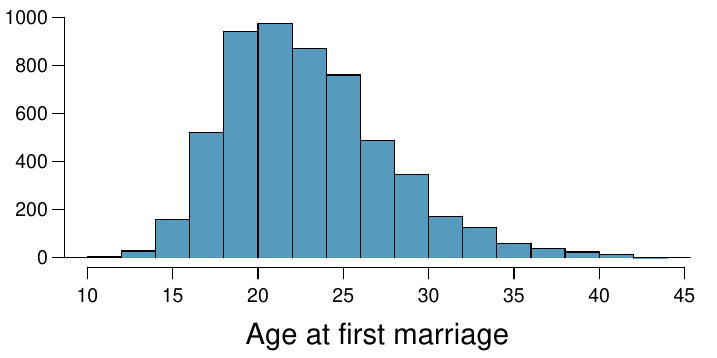
\includegraphics{./figs/marriage.png}
\caption{age at first marriage}
\end{figure}

Estimate the average age at first marriage of women

\begin{itemize}
\tightlist
\item
  using a 95\% confidence interval,

  \begin{itemize}
  \tightlist
  \item
    and interpret this interval in context.
  \end{itemize}
\item
  Discuss any relevant assumptions.
\end{itemize}

\begin{Shaded}
\begin{Highlighting}[]
\NormalTok{n }\OtherTok{\textless{}{-}} \DecValTok{5534}
\NormalTok{exp }\OtherTok{\textless{}{-}} \FloatTok{23.44}
\NormalTok{sd }\OtherTok{\textless{}{-}} \FloatTok{4.72}
\NormalTok{conf\_lvl }\OtherTok{\textless{}{-}} \FloatTok{0.95}
\NormalTok{sig\_lvl }\OtherTok{\textless{}{-}}\NormalTok{ (}\DecValTok{1} \SpecialCharTok{{-}}\NormalTok{ conf\_lvl) }\SpecialCharTok{/} \DecValTok{2}
\NormalTok{denom  }\OtherTok{\textless{}{-}}\NormalTok{ sd }\SpecialCharTok{/} \FunctionTok{sqrt}\NormalTok{(n)}
\NormalTok{z }\OtherTok{\textless{}{-}} \FunctionTok{qnorm}\NormalTok{(sig\_lvl, }\AttributeTok{lower.tail =}\NormalTok{ F)}
\NormalTok{e }\OtherTok{\textless{}{-}}\NormalTok{ z }\SpecialCharTok{*}\NormalTok{ denom}

\FunctionTok{c}\NormalTok{(exp }\SpecialCharTok{{-}}\NormalTok{ e, exp }\SpecialCharTok{+}\NormalTok{ e)}
\end{Highlighting}
\end{Shaded}

\begin{verbatim}
## [1] 23.31564 23.56436
\end{verbatim}

\hypertarget{answers}{%
\subsection{ANSWERS:}\label{answers}}

Distribution is symmetric, slightly skewed to the left, but that's fine.
From the data given: CI is calculated to be {[}23.32, 23.56{]}. With
95\% confidence we can say that the average age at first marriage of
women is 23 years old (23.32, 23.56).

\begin{center}\rule{0.5\linewidth}{0.5pt}\end{center}

\hypertarget{tidy-data-wrangling-2-pts}{%
\section{4. Tidy Data Wrangling (2
pts)}\label{tidy-data-wrangling-2-pts}}

This question uses a dataset from a case-control study of (o)esophageal
cancer in Ille-et-Vilaine, France.

This dataset is relatively clean, but there are some adjustments that we
would like to make to make it more readable for us to answer questions.

Some issues with the data might be left over from the method of data
entry

\begin{itemize}
\tightlist
\item
  remove the inconsistent ``g/day'' text from each entry that has it
\item
  \emph{without} removing the whole observation or that specific
  predictor
\end{itemize}

Let's only deal with bounded values

\begin{itemize}
\tightlist
\item
  remove the age group 75+
\item
  remove the alcohol group 120+
\item
  remove the tobacco group 30+
\end{itemize}

The question we want to answer is: do groups with higher levels of daily
tobacco consumption have higher occurrences of (o)esopheageal cancer?

Which tobacco group (not including 75+) has the highest occurrence of
(o)esophageal cancer?

We'll answer this by using \(\frac{ncases}{ncontrols}\), which we'll
call occurrence percentage

Calculate occurrence percentage for each age group summarize this in a
table

\begin{Shaded}
\begin{Highlighting}[]
\FunctionTok{library}\NormalTok{(tidyverse)}
\end{Highlighting}
\end{Shaded}

\begin{verbatim}
## -- Attaching packages --------------------------------------- tidyverse 1.3.2 --
## v ggplot2 3.4.0      v purrr   0.3.5 
## v tibble  3.1.8      v dplyr   1.0.10
## v tidyr   1.2.1      v stringr 1.4.1 
## v readr   2.1.3      v forcats 0.5.2 
## -- Conflicts ------------------------------------------ tidyverse_conflicts() --
## x dplyr::filter() masks stats::filter()
## x dplyr::lag()    masks stats::lag()
\end{verbatim}

\begin{Shaded}
\begin{Highlighting}[]
\FunctionTok{data}\NormalTok{(esoph)}

\NormalTok{esoph\_filtered }\OtherTok{\textless{}{-}}\NormalTok{ esoph[esoph}\SpecialCharTok{$}\NormalTok{agegp }\SpecialCharTok{!=} \StringTok{"75+"} \SpecialCharTok{\&}\NormalTok{ esoph}\SpecialCharTok{$}\NormalTok{alcgp }\SpecialCharTok{!=} \StringTok{"120+"} \SpecialCharTok{\&}\NormalTok{ esoph}\SpecialCharTok{$}\NormalTok{tobgp }\SpecialCharTok{!=} \StringTok{"30+"}\NormalTok{, }
\NormalTok{                        ] }\SpecialCharTok{\%\textgreater{}\%} \FunctionTok{mutate}\NormalTok{(}\AttributeTok{alcgp =} \FunctionTok{gsub}\NormalTok{(}\StringTok{"g/day"}\NormalTok{, }\StringTok{""}\NormalTok{, alcgp), }
                                     \AttributeTok{tobgp =} \FunctionTok{gsub}\NormalTok{(}\StringTok{"g/day"}\NormalTok{, }\StringTok{""}\NormalTok{, tobgp))}

\NormalTok{esoph\_filtered }\SpecialCharTok{\%\textgreater{}\%} \FunctionTok{group\_by}\NormalTok{(tobgp}
\NormalTok{             ) }\SpecialCharTok{\%\textgreater{}\%} \FunctionTok{summarize}\NormalTok{(}\AttributeTok{mean\_cases =} \FunctionTok{mean}\NormalTok{(ncases),}
                             \AttributeTok{sd\_cases =} \FunctionTok{sd}\NormalTok{(ncases),}
                             \AttributeTok{mean\_controls =} \FunctionTok{mean}\NormalTok{(ncontrols),}
                             \AttributeTok{sd\_controls =} \FunctionTok{sd}\NormalTok{(ncontrols))}
\end{Highlighting}
\end{Shaded}

\begin{verbatim}
## # A tibble: 3 x 5
##   tobgp mean_cases sd_cases mean_controls sd_controls
##   <chr>      <dbl>    <dbl>         <dbl>       <dbl>
## 1 0-9         3.87     4.91          27.9       17.4 
## 2 10-19       2.8      2.60          11.1        5.62
## 3 20-29       1.86     1.88           6.5        3.92
\end{verbatim}

\hypertarget{answers-from-the-summary-statistics-of-both-case-and-controls-grouped-by-tobacco-consumption-as-the-tobacco-consumption-increases-the-number-of-cases-as-well-as-controls-of-oesophageal-cancer-decreases-with-the-lowest-level-of-tobacco-consumption-having-the-highest-mean-occurences}{%
\subsection{ANSWERS: from the summary statistics of both case and
controls grouped by tobacco consumption, as the tobacco consumption
increases, the number of cases as well as controls of (o)esophageal
cancer decreases, with the lowest level of tobacco consumption having
the highest mean
occurences}\label{answers-from-the-summary-statistics-of-both-case-and-controls-grouped-by-tobacco-consumption-as-the-tobacco-consumption-increases-the-number-of-cases-as-well-as-controls-of-oesophageal-cancer-decreases-with-the-lowest-level-of-tobacco-consumption-having-the-highest-mean-occurences}}

\begin{center}\rule{0.5\linewidth}{0.5pt}\end{center}

\hypertarget{eda-summary-stats-visualization-3-pts}{%
\section{5. EDA, Summary Stats \& Visualization (3
pts)}\label{eda-summary-stats-visualization-3-pts}}

For this question, we'll look at some classical Michelson data from 1879
on the speed of light.

The data consists of 5 experiments, each with 20 consecutive runs with a
speed of light measurement for each run (km/sec, with 299000
subtracted).

We want to compare the different experiments using visualizations and
summary statistics.

5.a) Create a table reporting summary statistics for each experiment.

And report the following: variance, standard deviation, mean, maximum

5.b) Create visualizations comparing the different experiments

\begin{itemize}
\tightlist
\item
  how is the data in each experiment distributed?

  \begin{itemize}
  \tightlist
  \item
    (justify using at least one plot)
  \end{itemize}
\item
  use a box and whisker plot to compare the means and distributions
\end{itemize}

\begin{Shaded}
\begin{Highlighting}[]
\FunctionTok{data}\NormalTok{(morley)}
\end{Highlighting}
\end{Shaded}

\hypertarget{answer-5.a}{%
\subsection{ANSWER 5.a)}\label{answer-5.a}}

\begin{Shaded}
\begin{Highlighting}[]
\FunctionTok{library}\NormalTok{(dplyr)}
\NormalTok{morley}\SpecialCharTok{$}\NormalTok{Expt }\OtherTok{\textless{}{-}} \FunctionTok{as.factor}\NormalTok{(morley}\SpecialCharTok{$}\NormalTok{Expt)}

\NormalTok{stats\_by\_expt }\OtherTok{\textless{}{-}}\NormalTok{ morley }\SpecialCharTok{\%\textgreater{}\%} \FunctionTok{group\_by}\NormalTok{(Expt}
\NormalTok{                      ) }\SpecialCharTok{\%\textgreater{}\%} \FunctionTok{summarize}\NormalTok{(}\AttributeTok{mean =} \FunctionTok{mean}\NormalTok{(Speed), }
                                      \AttributeTok{var =} \FunctionTok{var}\NormalTok{(Speed), }
                                      \AttributeTok{sd =} \FunctionTok{sd}\NormalTok{(Speed), }
                                      \AttributeTok{max =} \FunctionTok{max}\NormalTok{(Speed))}

\NormalTok{stats\_by\_expt}
\end{Highlighting}
\end{Shaded}

\begin{verbatim}
## # A tibble: 5 x 5
##   Expt   mean    var    sd   max
##   <fct> <dbl>  <dbl> <dbl> <int>
## 1 1      909  11009. 105.   1070
## 2 2      856   3741.  61.2   960
## 3 3      845   6258.  79.1   970
## 4 4      820.  3605   60.0   920
## 5 5      832.  2940.  54.2   950
\end{verbatim}

\hypertarget{answer-5.b}{%
\subsection{ANSWER 5.b)}\label{answer-5.b}}

\begin{Shaded}
\begin{Highlighting}[]
\FunctionTok{library}\NormalTok{(ggplot2)}

\FunctionTok{ggplot}\NormalTok{(}\AttributeTok{data =}\NormalTok{ morley,}
       \AttributeTok{mapping =} \FunctionTok{aes}\NormalTok{(}\AttributeTok{x =}\NormalTok{ Speed, }\AttributeTok{fill =}\NormalTok{ Expt)}
\NormalTok{       ) }\SpecialCharTok{+} \FunctionTok{geom\_histogram}\NormalTok{(}\AttributeTok{position =} \StringTok{"identity"}
\NormalTok{       ) }\SpecialCharTok{+} \FunctionTok{ggtitle}\NormalTok{(}\StringTok{"Frequency of Speed by Experiment"}\NormalTok{)}
\end{Highlighting}
\end{Shaded}

\begin{verbatim}
## `stat_bin()` using `bins = 30`. Pick better value with `binwidth`.
\end{verbatim}

\begin{center}\includegraphics{2208-DSCI351-251m-451-FinalExam-MXD601_files/figure-latex/unnamed-chunk-9-1} \end{center}

\begin{Shaded}
\begin{Highlighting}[]
\FunctionTok{ggplot}\NormalTok{(}\AttributeTok{data =} \FunctionTok{subset}\NormalTok{(morley, Expt }\SpecialCharTok{==} \DecValTok{1}\NormalTok{),}
       \AttributeTok{mapping =} \FunctionTok{aes}\NormalTok{(}\AttributeTok{x =}\NormalTok{ Speed)}
\NormalTok{       ) }\SpecialCharTok{+} \FunctionTok{geom\_histogram}\NormalTok{(}\AttributeTok{position =} \StringTok{"identity"}
\NormalTok{       ) }\SpecialCharTok{+} \FunctionTok{ggtitle}\NormalTok{(}\StringTok{"Frequency of Speed (Expt 1)"}\NormalTok{)}
\end{Highlighting}
\end{Shaded}

\begin{verbatim}
## `stat_bin()` using `bins = 30`. Pick better value with `binwidth`.
\end{verbatim}

\begin{center}\includegraphics{2208-DSCI351-251m-451-FinalExam-MXD601_files/figure-latex/unnamed-chunk-9-2} \end{center}

\begin{Shaded}
\begin{Highlighting}[]
\FunctionTok{ggplot}\NormalTok{(}\AttributeTok{data =} \FunctionTok{subset}\NormalTok{(morley, Expt }\SpecialCharTok{==} \DecValTok{2}\NormalTok{),}
       \AttributeTok{mapping =} \FunctionTok{aes}\NormalTok{(}\AttributeTok{x =}\NormalTok{ Speed)}
\NormalTok{       ) }\SpecialCharTok{+} \FunctionTok{geom\_histogram}\NormalTok{(}\AttributeTok{position =} \StringTok{"identity"}
\NormalTok{       ) }\SpecialCharTok{+} \FunctionTok{ggtitle}\NormalTok{(}\StringTok{"Frequency of Speed (Expt 2)"}\NormalTok{)}
\end{Highlighting}
\end{Shaded}

\begin{verbatim}
## `stat_bin()` using `bins = 30`. Pick better value with `binwidth`.
\end{verbatim}

\begin{center}\includegraphics{2208-DSCI351-251m-451-FinalExam-MXD601_files/figure-latex/unnamed-chunk-9-3} \end{center}

\begin{Shaded}
\begin{Highlighting}[]
\FunctionTok{ggplot}\NormalTok{(}\AttributeTok{data =} \FunctionTok{subset}\NormalTok{(morley, Expt }\SpecialCharTok{==} \DecValTok{3}\NormalTok{),}
       \AttributeTok{mapping =} \FunctionTok{aes}\NormalTok{(}\AttributeTok{x =}\NormalTok{ Speed)}
\NormalTok{       ) }\SpecialCharTok{+} \FunctionTok{geom\_histogram}\NormalTok{(}\AttributeTok{position =} \StringTok{"identity"}
\NormalTok{       ) }\SpecialCharTok{+} \FunctionTok{ggtitle}\NormalTok{(}\StringTok{"Frequency of Speed (Expt 3)"}\NormalTok{)}
\end{Highlighting}
\end{Shaded}

\begin{verbatim}
## `stat_bin()` using `bins = 30`. Pick better value with `binwidth`.
\end{verbatim}

\begin{center}\includegraphics{2208-DSCI351-251m-451-FinalExam-MXD601_files/figure-latex/unnamed-chunk-9-4} \end{center}

\begin{Shaded}
\begin{Highlighting}[]
\FunctionTok{ggplot}\NormalTok{(}\AttributeTok{data =} \FunctionTok{subset}\NormalTok{(morley, Expt }\SpecialCharTok{==} \DecValTok{4}\NormalTok{),}
       \AttributeTok{mapping =} \FunctionTok{aes}\NormalTok{(}\AttributeTok{x =}\NormalTok{ Speed)}
\NormalTok{       ) }\SpecialCharTok{+} \FunctionTok{geom\_histogram}\NormalTok{(}\AttributeTok{position =} \StringTok{"identity"}
\NormalTok{       ) }\SpecialCharTok{+} \FunctionTok{ggtitle}\NormalTok{(}\StringTok{"Frequency of Speed (Expt 4)"}\NormalTok{)}
\end{Highlighting}
\end{Shaded}

\begin{verbatim}
## `stat_bin()` using `bins = 30`. Pick better value with `binwidth`.
\end{verbatim}

\begin{center}\includegraphics{2208-DSCI351-251m-451-FinalExam-MXD601_files/figure-latex/unnamed-chunk-9-5} \end{center}

\begin{Shaded}
\begin{Highlighting}[]
\FunctionTok{ggplot}\NormalTok{(}\AttributeTok{data =} \FunctionTok{subset}\NormalTok{(morley, Expt }\SpecialCharTok{==} \DecValTok{5}\NormalTok{),}
       \AttributeTok{mapping =} \FunctionTok{aes}\NormalTok{(}\AttributeTok{x =}\NormalTok{ Speed)}
\NormalTok{       ) }\SpecialCharTok{+} \FunctionTok{geom\_histogram}\NormalTok{(}\AttributeTok{position =} \StringTok{"identity"}
\NormalTok{       ) }\SpecialCharTok{+} \FunctionTok{ggtitle}\NormalTok{(}\StringTok{"Frequency of Speed (Expt 5)"}\NormalTok{)}
\end{Highlighting}
\end{Shaded}

\begin{verbatim}
## `stat_bin()` using `bins = 30`. Pick better value with `binwidth`.
\end{verbatim}

\begin{center}\includegraphics{2208-DSCI351-251m-451-FinalExam-MXD601_files/figure-latex/unnamed-chunk-9-6} \end{center}

\begin{Shaded}
\begin{Highlighting}[]
\FunctionTok{ggplot}\NormalTok{(}\AttributeTok{data =}\NormalTok{ morley,}
       \AttributeTok{mapping =} \FunctionTok{aes}\NormalTok{(}\AttributeTok{x =}\NormalTok{ Run, }
                     \AttributeTok{y =}\NormalTok{ Speed, }
                     \AttributeTok{group =}\NormalTok{ Expt, }
                     \AttributeTok{color =}\NormalTok{ Expt, }
                     \AttributeTok{fill =}\NormalTok{ Expt)}
\NormalTok{       ) }\SpecialCharTok{+} \FunctionTok{geom\_point}\NormalTok{(}
\NormalTok{       ) }\SpecialCharTok{+} \FunctionTok{geom\_line}\NormalTok{(}
\NormalTok{       ) }\SpecialCharTok{+} \FunctionTok{ggtitle}\NormalTok{(}\StringTok{"Speed over Run by Experiment"}\NormalTok{)}
\end{Highlighting}
\end{Shaded}

\begin{center}\includegraphics{2208-DSCI351-251m-451-FinalExam-MXD601_files/figure-latex/unnamed-chunk-9-7} \end{center}

\begin{Shaded}
\begin{Highlighting}[]
\FunctionTok{ggplot}\NormalTok{(}\AttributeTok{data =}\NormalTok{ morley, }\FunctionTok{aes}\NormalTok{(}\AttributeTok{x =}\NormalTok{ Expt, }
                          \AttributeTok{y =}\NormalTok{ Speed)}
\NormalTok{       ) }\SpecialCharTok{+} \FunctionTok{geom\_boxplot}\NormalTok{(}\FunctionTok{aes}\NormalTok{(}\AttributeTok{color =}\NormalTok{ Expt), }
                        \AttributeTok{show.legend =} \ConstantTok{TRUE}
\NormalTok{       ) }\SpecialCharTok{+} \FunctionTok{labs}\NormalTok{(}\AttributeTok{x =} \StringTok{"Experiment"}\NormalTok{,}
                \AttributeTok{y =} \StringTok{"Speed"}\NormalTok{,}
                \AttributeTok{color =} \StringTok{"Expt"}
\NormalTok{       ) }\SpecialCharTok{+} \FunctionTok{ggtitle}\NormalTok{(}\StringTok{"Speed Summaries by Experiment"}\NormalTok{)}
\end{Highlighting}
\end{Shaded}

\begin{center}\includegraphics{2208-DSCI351-251m-451-FinalExam-MXD601_files/figure-latex/unnamed-chunk-9-8} \end{center}

Experiment 1 is skewed to the right, 2 and 3 as well, 4 is oscillating,
5 looks to be in the middle. 3 suffers from a massive speed drop between
runs 4 and 7; goes back up instantaneously in runs 8-10. 1 kind of does
the same thing between 10-15, and 1-5. 2 looks to be the most
consistent, coming right after 2 is 4 and 5. 1 has the highest mean, 5
has the lowest, but it's strongly leaning to the lower half of the data.

\begin{center}\rule{0.5\linewidth}{0.5pt}\end{center}

\hypertarget{what-is-data-science-5-paragraph-essay-with-citations-4-pts}{%
\section{6. What is data science? (5 paragraph essay with citations) (4
pts)}\label{what-is-data-science-5-paragraph-essay-with-citations-4-pts}}

What do you find most interesting or exciting

\begin{itemize}
\tightlist
\item
  about data science and EDA?
\item
  What defines data science and how has it come about.\\
\item
  What are its characteristics, and what are the elements of

  \begin{itemize}
  \tightlist
  \item
    a data science tool chain,
  \item
    a data science pipeline, and
  \item
    a data analysis.
  \end{itemize}
\end{itemize}

Use the structure of a 5 paragraph essay

\begin{itemize}
\tightlist
\item
  (Introduction, 3 topic paragraphs, 1 concluding paragraph)
\item
  with citations/references.
\end{itemize}

\hypertarget{data-science-experience}{%
\subsubsection{Data Science Experience}\label{data-science-experience}}

Data Science is the science encapsulating the processing of data to
generate new information or gain more knowledge about the data in
general, to be able to classify it and generalize it as a whole, or
infer new things in the future, or whatever else the purpose handling
the data is supposed to achieve. Data analysis can be done in 2 ways,
one of them being more dominant than the other, and the other to
characterize certain models together. Exploratory Data Science is a bit
more dominant or powerful to explore new ways to analyze the data,
whereas utilizing ML Algorithms and Statistical Models helps to automate
the process we have already discovered (in a way, not entirely). I've
taken two courses alongside this course this semester, where one heavily
influences and transform the data analysis process (AI), and one that
uses it to protect digital systems (Cybersecurity).

A common concept that went through discussion is, ``what do we do with
the information we obtain, and how do we interpret it?'' The data
science process is as follows: 1 - Data Collection Process: get raw data
from the real world, reformat and process the data, clean the data; 2 -
Data Analysis Process: perform data analysis on it (either EDA or ML
Algos/Stat Models). If the data is not sufficient in the Data Analysis
Process, go back to the Data Collection Process. Rinse and repeat
between these 2 processes until we can clearly and confidently
communicate/visualize/report our findings to the world. From these
findings, we can build products based on this analysis that can help
better the world.

The data scientist must ask, ``What data needs to be collected? What do
I want it to look like? What question am I supposed to answer with this?
Why am I doing this?'', and formulate hypothesis, try again frequently,
until there is a new concrete idea has emerged from this analysis that
can simplify the data to something more comprehensible, concise, and
potentially reusable under similar conditions of data (which then become
statistical models) {[}1{]}. This idea and the models can then be used
to create or automate processes of data handling and processing, quickly
determining validity of data, etc.

Something I learned from using this process is to delete faulty records
from a database in some database tables. I used the DSCI process to
collect, process, interpret, and rinse and repeat for the duration of
this semester until I finally was able to create a model, a set of
queries, that can fix this faulty data in the database to ensure proper
history and record keeping of the data records over the course of their
lifetime. I especially used EDA in this context, because some data
cannot be fit into certain models, and for this, we have to explore (the
understanding of the problem that is trying to be solved changes as time
passes) and traverse the data until we can properly understand what it's
trying to say and generalize it under a certain train of thought.

EDA is the willingness to look for things we do and do not believe to be
there. There is no hypothesis, no model.So what we do is systematically
go through the data, use plots (plot distributions, time series),
transform the variables to look into PAIRWISE relationships between the
variables, and generate summary statistics (mean, min, max, quartiles,
and outliers). Ultimately, the data is NOT the objective, modeling and
TIDY data helps, but understanding using the data to represent some
aspect of reality is what's important {[}1{]}.

1 - {[}/2-class/2208-351-351m-451-w05b-f2-Inference-DSCIprocess{]}

\begin{center}\rule{0.5\linewidth}{0.5pt}\end{center}

\hypertarget{eda-of-tco-degradation-4-pts}{%
\section{7. EDA of TCO degradation (4
pts)}\label{eda-of-tco-degradation-4-pts}}

This problem will be similar to the LE3 on Degradation of Hard Coat
Acrylics.

\begin{itemize}
\tightlist
\item
  But you are given a \texttt{.csv} file of a clean and tidy data set.
\item
  You will need to do EDA and make figures and summaries of what you
  find.
\item
  And list the insights you can develop from your EDA.
\item
  The \texttt{.csv} datafile is located in the data subfolder of the
  \texttt{exam-final}
\end{itemize}

TCO's are transparent conductive oxides

\begin{itemize}
\tightlist
\item
  Such as ITO, AZO and FTO.
\item
  Heather Lemire Mirletz did her MS thesis on these
\item
  and has a journal paper being published.
\end{itemize}

Here is the abstract of the paper

\begin{figure}
\centering

\includegraphics{./figs/tco-degr.png}
\caption{tco-degr abstract}
\end{figure}

Here is a mindmap of her data science study

\begin{figure}
\centering
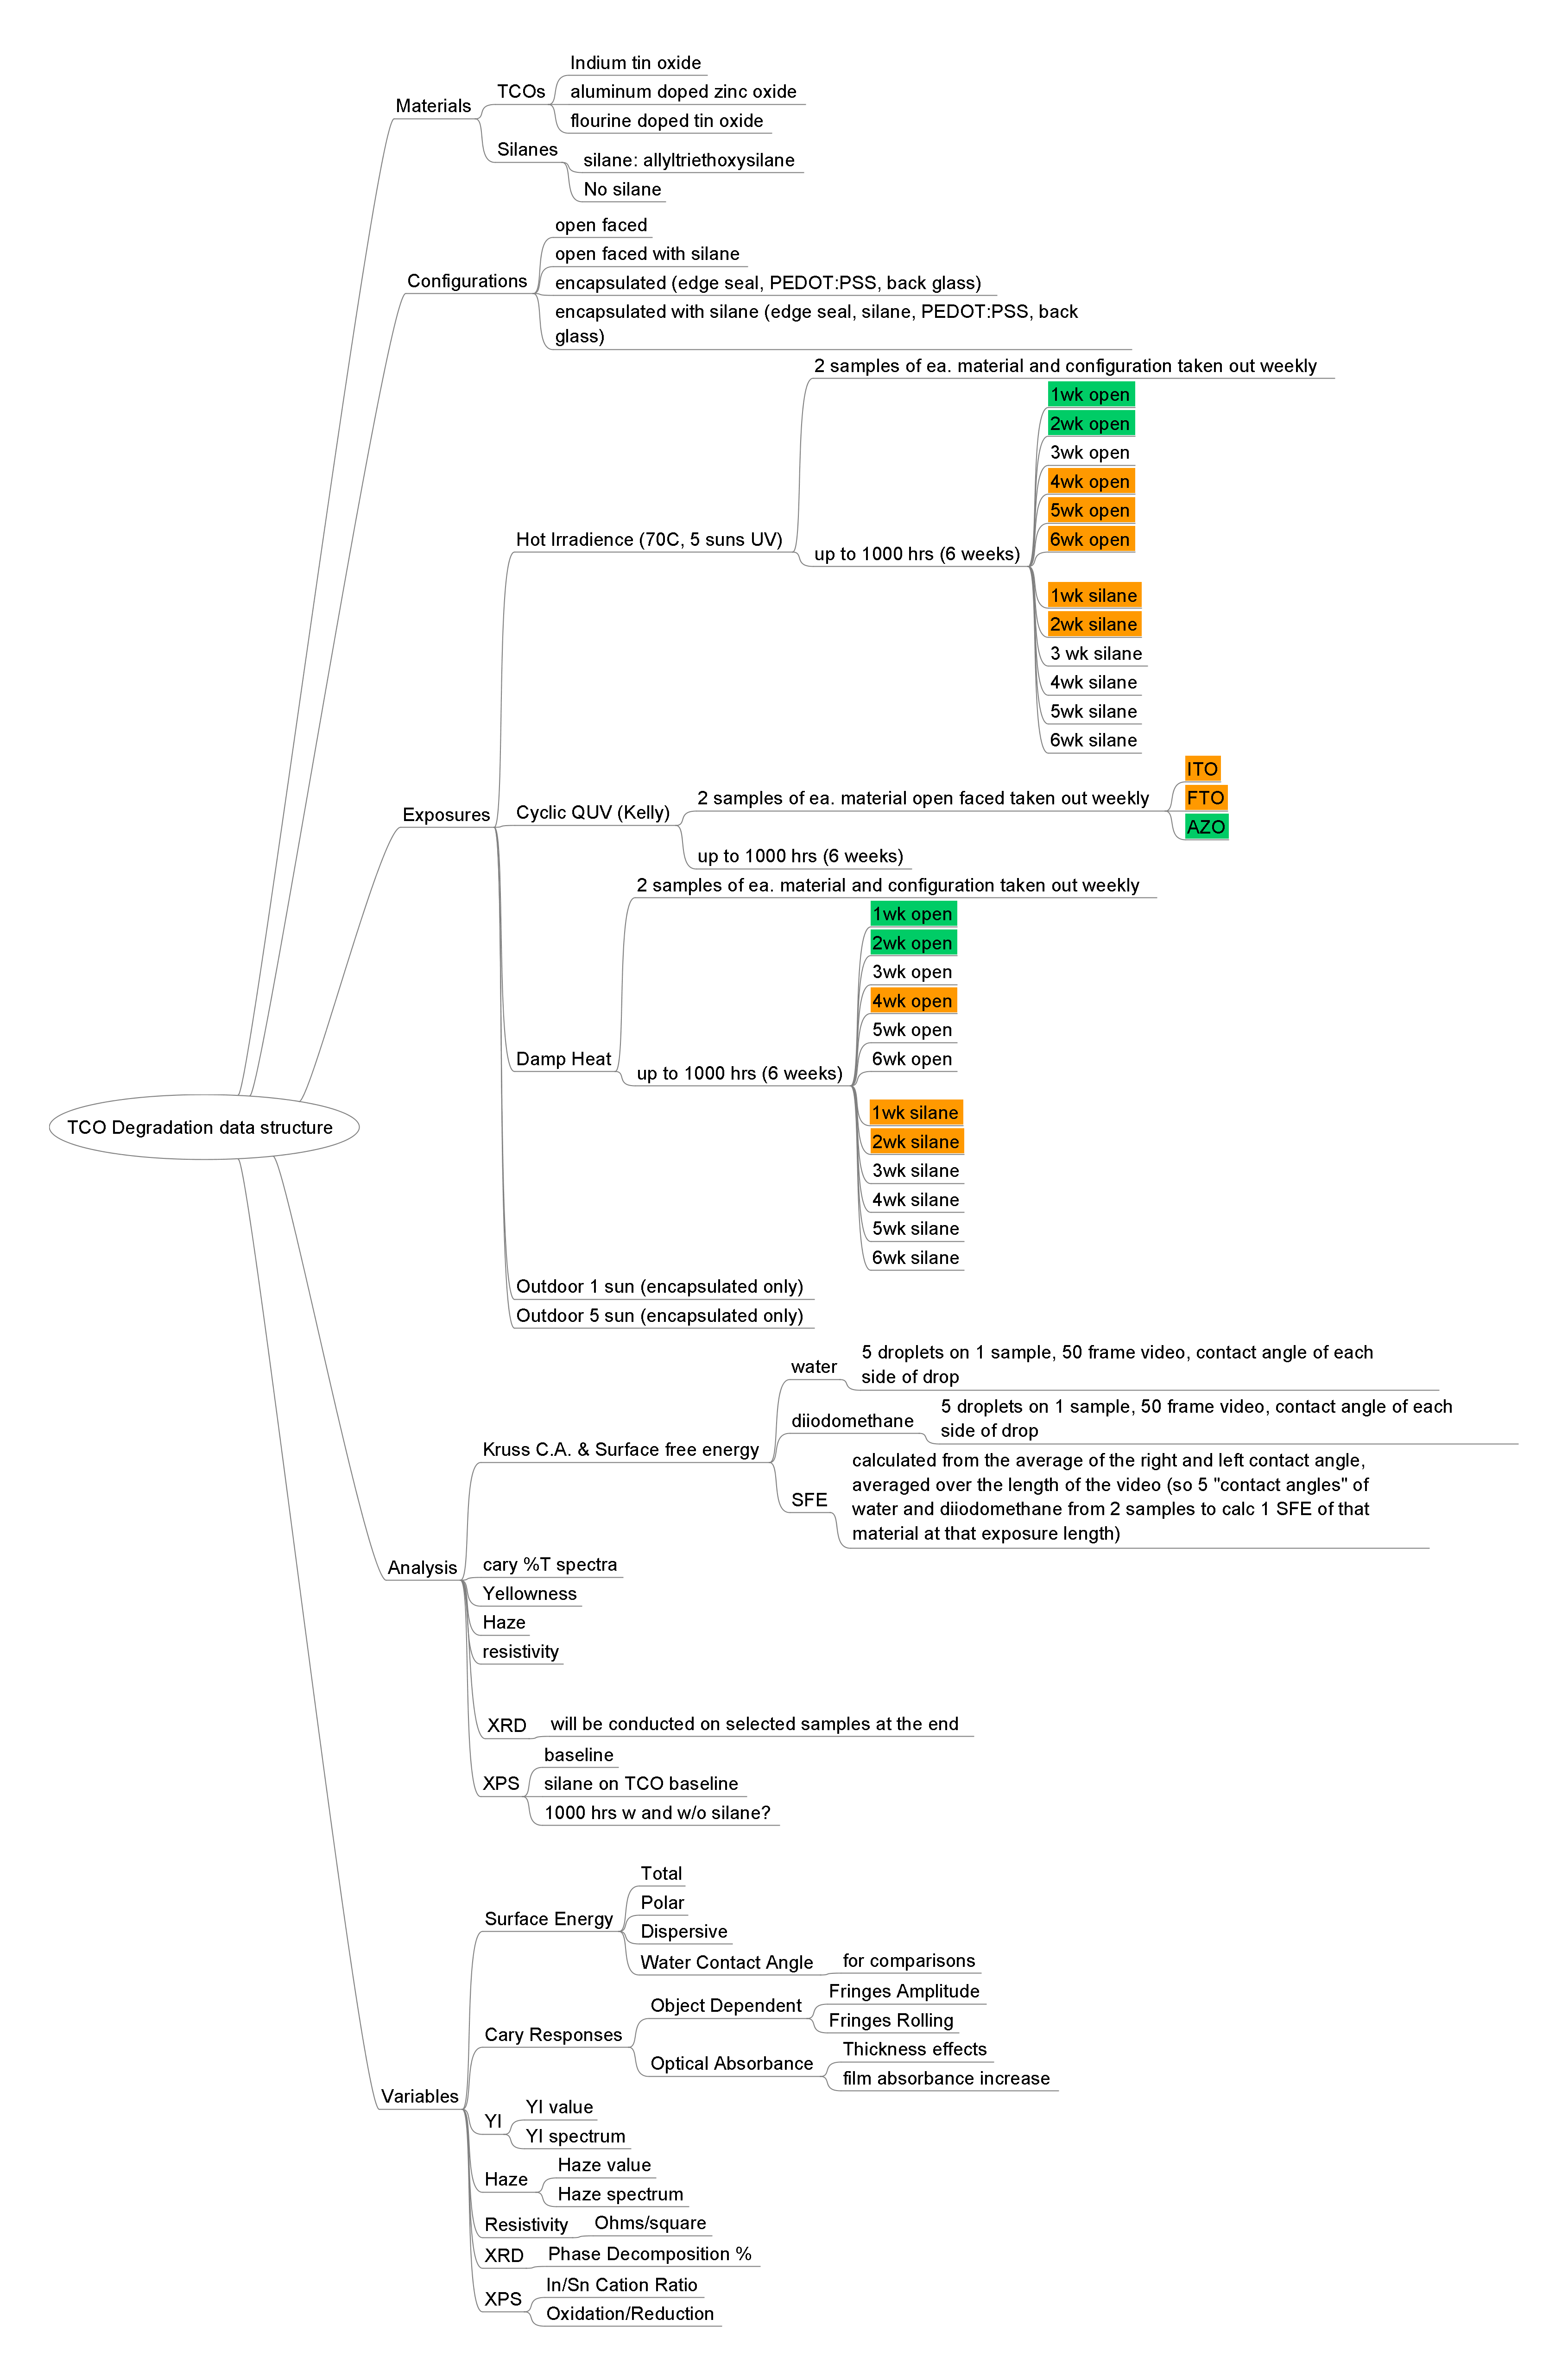
\includegraphics{./figs/tcoDataStructure.png}
\caption{tco-DataStructue}
\end{figure}

Here is information on the samples studied

\begin{figure}
\centering
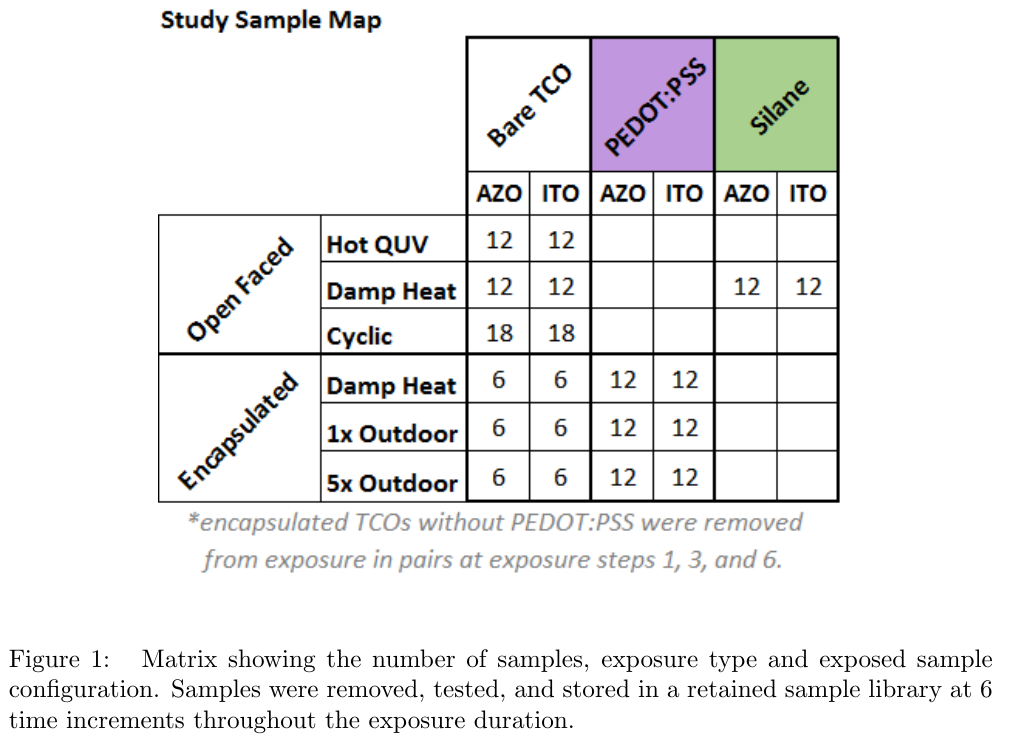
\includegraphics{./figs/tco-samples.png}
\caption{tco-samples}
\end{figure}

Here is information about the exposures she did

\begin{figure}
\centering
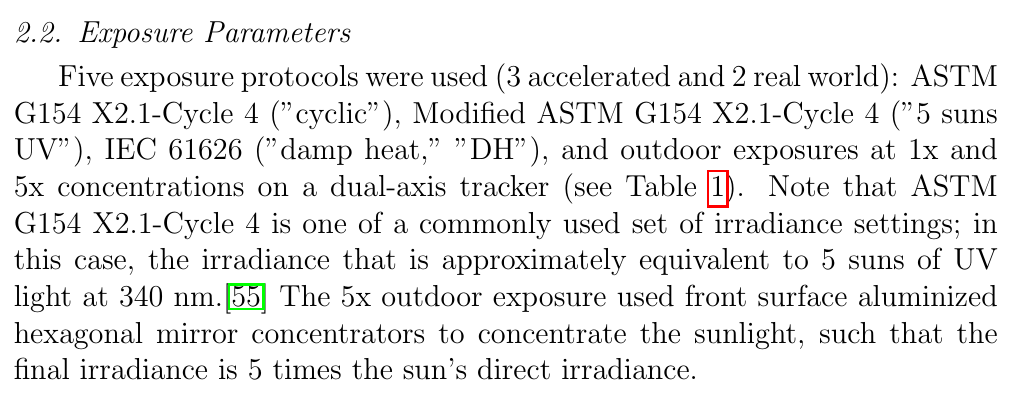
\includegraphics{./figs/tco-exposures.png}
\caption{tco-exposures}
\end{figure}

And a table about the exposures

\begin{figure}
\centering
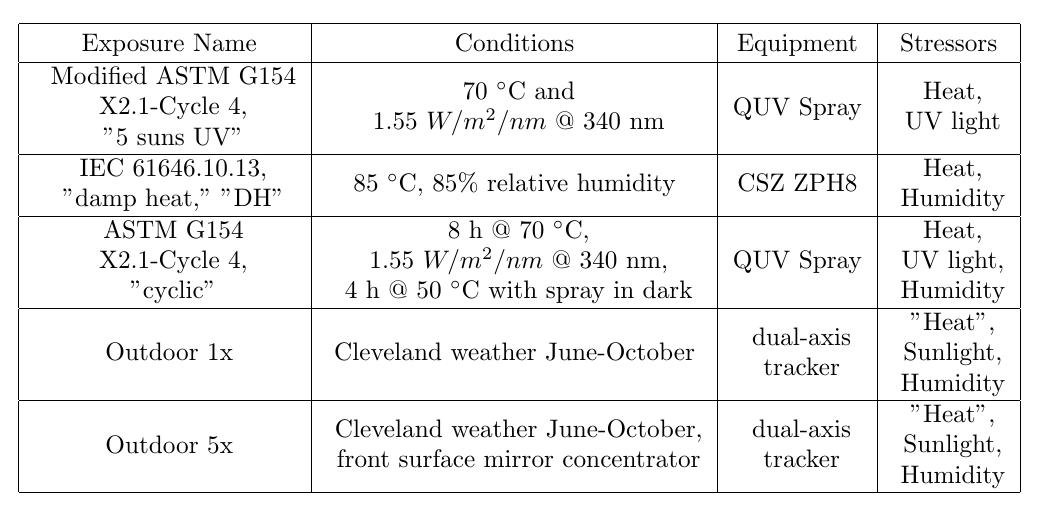
\includegraphics{./figs/tco-exposures2.png}
\caption{tco-exposures2}
\end{figure}

Some questions to try to address, showing your results.

\begin{itemize}
\tightlist
\item
  7.a) Which type of TCO (ITO, AZO, FTO) is most stable?
\item
  7.b) Which type of Exposure is most aggressive?
\item
  7.c) How do open vs.~encapsulated samples compare.
\item
  7.d) What other insights can you identify and demonstrate from your
  EDA?
\end{itemize}

\begin{Shaded}
\begin{Highlighting}[]
\NormalTok{exposures }\OtherTok{\textless{}{-}} \FunctionTok{read.csv}\NormalTok{(}\StringTok{\textquotesingle{}data/TCOs.csv\textquotesingle{}}\NormalTok{)}
\NormalTok{exposures }\OtherTok{\textless{}{-}}\NormalTok{ exposures[}\SpecialCharTok{!}\NormalTok{(}\FunctionTok{is.na}\NormalTok{(exposures}\SpecialCharTok{$}\NormalTok{SFEtot)), ]}
\end{Highlighting}
\end{Shaded}

ANSWERS:

\hypertarget{answer-7.a}{%
\subsection{ANSWER 7.a)}\label{answer-7.a}}

\begin{Shaded}
\begin{Highlighting}[]
\NormalTok{stats\_by\_TCO }\OtherTok{\textless{}{-}}\NormalTok{ exposures }\SpecialCharTok{\%\textgreater{}\%} \FunctionTok{group\_by}\NormalTok{(MaterialType}
\NormalTok{                      ) }\SpecialCharTok{\%\textgreater{}\%} \FunctionTok{summarize}\NormalTok{(}\AttributeTok{mean =} \FunctionTok{mean}\NormalTok{(SFEtot), }
                                      \AttributeTok{sd =} \FunctionTok{sd}\NormalTok{(SFEtot))}
\NormalTok{stats\_by\_TCO}
\end{Highlighting}
\end{Shaded}

\begin{verbatim}
## # A tibble: 3 x 3
##   MaterialType  mean    sd
##   <chr>        <dbl> <dbl>
## 1 AZO           78.5 10.4 
## 2 FTO           80.4  2.47
## 3 ITO           72.3  9.56
\end{verbatim}

FTO is most stable

\hypertarget{answer-7.b}{%
\subsection{ANSWER 7.b)}\label{answer-7.b}}

\begin{Shaded}
\begin{Highlighting}[]
\NormalTok{stats\_by\_exposure }\OtherTok{\textless{}{-}}\NormalTok{ exposures }\SpecialCharTok{\%\textgreater{}\%} \FunctionTok{group\_by}\NormalTok{(ExposureType}
\NormalTok{                      ) }\SpecialCharTok{\%\textgreater{}\%} \FunctionTok{summarize}\NormalTok{(}\AttributeTok{mean =} \FunctionTok{mean}\NormalTok{(SFEtot),}
                                      \AttributeTok{sd =} \FunctionTok{sd}\NormalTok{(SFEtot))}
\NormalTok{stats\_by\_exposure}
\end{Highlighting}
\end{Shaded}

\begin{verbatim}
## # A tibble: 3 x 3
##   ExposureType  mean    sd
##   <chr>        <dbl> <dbl>
## 1 Cyclic        82.8  1.65
## 2 DampHeat      72.7 12.8 
## 3 HotQUV        78.1  3.67
\end{verbatim}

Cyclic is most aggresive

\hypertarget{answer-7.c}{%
\subsection{ANSWER 7.c)}\label{answer-7.c}}

\begin{Shaded}
\begin{Highlighting}[]
\NormalTok{stats\_by\_silane }\OtherTok{\textless{}{-}}\NormalTok{ exposures }\SpecialCharTok{\%\textgreater{}\%} \FunctionTok{group\_by}\NormalTok{(Silane}
\NormalTok{                      ) }\SpecialCharTok{\%\textgreater{}\%} \FunctionTok{summarize}\NormalTok{(}\AttributeTok{mean =} \FunctionTok{mean}\NormalTok{(SFEtot),}
                                      \AttributeTok{sd =} \FunctionTok{sd}\NormalTok{(SFEtot))}
\NormalTok{stats\_by\_silane}
\end{Highlighting}
\end{Shaded}

\begin{verbatim}
## # A tibble: 2 x 3
##   Silane  mean    sd
##   <chr>  <dbl> <dbl>
## 1 No      80.6  2.68
## 2 Yes     65.4 13.5
\end{verbatim}

closed capsules have higher average and lower sd values than open ones

\hypertarget{answer-7.d}{%
\subsection{ANSWER 7.d)}\label{answer-7.d}}

couldn't finish this

\begin{center}\rule{0.5\linewidth}{0.5pt}\end{center}

\hypertarget{linear-regression-on-a-dataset-4-pts}{%
\section{8. Linear regression on a dataset (4
pts)}\label{linear-regression-on-a-dataset-4-pts}}

Here we'll use a base R dataset about vapor pressure to discuss the use
of linearity in science.

The Dataset contains 19 observations of temperature (Celsius) vs.~vapor
pressure (mmHg) for mercury

8.a) Start by plotting the data, temperature (x) vs.~vapor pressure (y).
This relationship is clearly not linear.

However, we may be able to pull a linear relationship from these two
metrics. A simplified form of the ``Antoine equation'' can be used to
model the relationship between temperature and vapor pressure:

\[log{P} = A - \frac{B}{T}\] - \(P\) is vapor pressure, \(T\) is
temperature - \(A\) and \(B\) are constants representing y intercept and
slope

Let's use this equation to fit our data with a linear model.

8.b) Mutate two new columns from the existing data, for \(log{P}\) and
for \(\frac{1}{T}\)

8.c) Create a linear model using lm() using the new columns as your
variables

8.d) Plot your linear model with \(log{P}\) and \(\frac{1}{T}\) axes

8.e) Report the results of your model (model summary) in a table

8.f) What are your approximations for \(A\) and \(B\) in the simplified
Antoine model using this data?

\begin{Shaded}
\begin{Highlighting}[]
\FunctionTok{data}\NormalTok{(pressure)}
\end{Highlighting}
\end{Shaded}

ANSWERS:

{[}if an answer is in your code block, put \texttt{\#\ a)} to show it in
your code{]}

\hypertarget{answer-8.a}{%
\subsection{ANSWER 8.a)}\label{answer-8.a}}

\begin{Shaded}
\begin{Highlighting}[]
\NormalTok{pressure }\OtherTok{\textless{}{-}}\NormalTok{ pressure[}\SpecialCharTok{{-}}\DecValTok{1}\NormalTok{, ]}
\FunctionTok{ggplot}\NormalTok{(pressure,}
       \FunctionTok{aes}\NormalTok{(}\AttributeTok{x =}\NormalTok{ temperature, }\AttributeTok{y =}\NormalTok{ pressure)}
\NormalTok{       ) }\SpecialCharTok{+} \FunctionTok{geom\_point}\NormalTok{(}
\NormalTok{       ) }\SpecialCharTok{+} \FunctionTok{geom\_line}\NormalTok{(}
\NormalTok{       )}
\end{Highlighting}
\end{Shaded}

\begin{center}\includegraphics{2208-DSCI351-251m-451-FinalExam-MXD601_files/figure-latex/unnamed-chunk-15-1} \end{center}

The plot indicates exponential growth between temperature and pressure

\hypertarget{answer-8.b}{%
\subsection{ANSWER 8.b)}\label{answer-8.b}}

\begin{Shaded}
\begin{Highlighting}[]
\NormalTok{pressure }\OtherTok{\textless{}{-}}\NormalTok{ pressure }\SpecialCharTok{\%\textgreater{}\%} \FunctionTok{mutate}\NormalTok{(}\AttributeTok{logp =} \FunctionTok{log}\NormalTok{(pressure), }\AttributeTok{frac =} \DecValTok{1} \SpecialCharTok{/}\NormalTok{ temperature)}
\end{Highlighting}
\end{Shaded}

\hypertarget{answer-8.c}{%
\subsection{ANSWER 8.c)}\label{answer-8.c}}

\begin{Shaded}
\begin{Highlighting}[]
\NormalTok{regress\_pressure }\OtherTok{\textless{}{-}} \FunctionTok{lm}\NormalTok{(logp }\SpecialCharTok{\textasciitilde{}}\NormalTok{ frac, pressure)}
\NormalTok{regress\_pressure}
\end{Highlighting}
\end{Shaded}

\begin{verbatim}
## 
## Call:
## lm(formula = logp ~ frac, data = pressure)
## 
## Coefficients:
## (Intercept)         frac  
##       4.484     -294.116
\end{verbatim}

\hypertarget{answer-8.d}{%
\subsection{ANSWER 8.d)}\label{answer-8.d}}

\begin{Shaded}
\begin{Highlighting}[]
\FunctionTok{ggplot}\NormalTok{(pressure,}
       \FunctionTok{aes}\NormalTok{(}\AttributeTok{x =}\NormalTok{ frac, }\AttributeTok{y =}\NormalTok{ logp)}
\NormalTok{       ) }\SpecialCharTok{+} \FunctionTok{geom\_point}\NormalTok{(}
\NormalTok{       ) }\SpecialCharTok{+} \FunctionTok{geom\_line}\NormalTok{(}
\NormalTok{       ) }\SpecialCharTok{+} \FunctionTok{geom\_smooth}\NormalTok{(}\AttributeTok{method =} \StringTok{"lm"}\NormalTok{)}
\end{Highlighting}
\end{Shaded}

\begin{verbatim}
## `geom_smooth()` using formula = 'y ~ x'
\end{verbatim}

\begin{center}\includegraphics{2208-DSCI351-251m-451-FinalExam-MXD601_files/figure-latex/unnamed-chunk-18-1} \end{center}

\hypertarget{answer-8.e}{%
\subsection{ANSWER 8.e)}\label{answer-8.e}}

\begin{Shaded}
\begin{Highlighting}[]
\FunctionTok{summary}\NormalTok{(regress\_pressure)}
\end{Highlighting}
\end{Shaded}

\begin{verbatim}
## 
## Call:
## lm(formula = logp ~ frac, data = pressure)
## 
## Residuals:
##     Min      1Q  Median      3Q     Max 
## -3.2153 -2.1272  0.0797  1.9102  3.4965 
## 
## Coefficients:
##              Estimate Std. Error t value Pr(>|t|)    
## (Intercept)    4.4838     0.7244   6.190 1.30e-05 ***
## frac        -294.1163    48.7312  -6.035 1.73e-05 ***
## ---
## Signif. codes:  0 '***' 0.001 '**' 0.01 '*' 0.05 '.' 0.1 ' ' 1
## 
## Residual standard error: 2.327 on 16 degrees of freedom
## Multiple R-squared:  0.6948, Adjusted R-squared:  0.6757 
## F-statistic: 36.43 on 1 and 16 DF,  p-value: 1.732e-05
\end{verbatim}

\hypertarget{answer-8.f}{%
\subsection{ANSWER 8.f)}\label{answer-8.f}}

y (logP) = b (A) + m (-B) x (1/T)

Intercept (A) = 4.48

Slope (B) = -294

The approximations A and B represent intercept and slope respectively
\_\_\_\_\_\_\_\_\_\_\_\_

\end{document}
